\documentclass[11pt]{article}

\usepackage{amsmath}
\usepackage{graphicx}
\usepackage{caption}
\usepackage{stix}

\setlength{\parindent}{0pt}
\graphicspath{ {images/} }

\begin{document}

\section{Kinematik}

\subsection{Momentane Geschwindigkeit}

Ableitung nach der Zeit t der Funktion $x(t)$
\begin{equation*}
	v(t) = \frac{dx}{dt}
\end{equation*}

\subsection{Momentane Beschleunigung}

Zweite Ableitung nach der Zeit $t$ der Funktion $x(t)$
\begin{equation*}
	a(t) = \frac{d^2x}{dt^2}
\end{equation*}

\subsection{Integration der Bewegung}

\begin{equation*}
	x(t) = \int_{t_0}^{t}v(u)du + x_0
\end{equation*}

$x(t)$ ist die Stammfunktion von $v(t)$. $x_0$ ist die zum Beispiel die Position des K{\"o}rpers zu einem bestimmten Anfangszeitpunkt.\newline
Falls Bewegung gleichf{\"o}rmig und geradlinig: $v(t) = konst. \Rightarrow a(t) = 0$ \newline
\begin{equation*}
	x(t) = x_0 + v_0(t - t_0)
\end{equation*}

Falls Bewegung gleichf{\"o}rmig beschleunigt und geradlinig: $a(t) = a_0 = konst.$ \newline
\begin{equation*}
\begin{split}
		v(t)& = v_0 + a_0(t - t_0)\\
	x(t)& = x_0 + v_0(t - t_0) + \frac{1}{2}a_0(t - t_0)^2
\end{split}
\end{equation*}

Spezialfall: $x_0 = v_0 = t_0 = 0$ \newline
\begin{equation*}
\begin{split}
	x(t)& = \frac{1}{2}a_0t^2 \\
	v(t)& = a_0t \\
	a(t)& = a_0
\end{split}
\end{equation*}

\subsection{Gravitation}
In der N{\"a}he der Erdoberfl{\"a}che f{\"u}hlt jeder K{\"o}per, ubabh{\"a}ngig von seinem Gewicht, dieselbe Beschleunigung (wenn der Luftwiderstand vernachl{\"a}ssigt wird).
\begin{equation*}
	h = \frac{1}{2}gt^2 \Rightarrow t = \sqrt{\frac{2h}{g}}
\end{equation*}

mit Fallh{\"o}he $h$ und Fallzeit $t$.

\subsection{Bahnkurve beim Ballwurf}

Zur Zeit $t_{max}$ erreicht die Kugel den h{\"o}chsten Punkt ihrer Bahnkurve. In diesem Punkt verschwindet die vertikale Geschwindigkeit:
\begin{equation*}
	t_{max} = \frac{v_{0y}}{g}
\end{equation*}

Die maximale H{\"o}he der Kugel ist:
\begin{equation*}
	y_{max} = y_0 + \frac{{v_{0y}}^2}{2g}
\end{equation*}

\subsection{Gleichf{\"o}rmige Kreisbewegung}

\begin{equation*}
	\varphi(t) = \omega t
\end{equation*}

mit Winkelgeschwindigkeit $\omega$ und Periode $T$:
\begin{equation*}
	\varphi(T) = 2 \pi \Rightarrow T = \frac{2 \pi}{\omega}
\end{equation*}

\subsubsection{Geschwindigkeitsvektor}
Betrag: $|\vec{v}| = r \omega = konst.$ \newline
Die Richtung der Geschwindigkeit ist senkrecht zum Ortsvektor.

\subsubsection{Beschleunigungsvektor}
Zeigt in Richtung Zentrum des Kreises mit Betrag: $\vec{a} = r \omega ^2 = \frac{v^2}{r}$

\section{Dynamik}

\subsection{Masse}
Astronaut in seiner Umlaufbahn um die Erde ist gewichtslos, aber nicht masselos.

Masse eines K{\"o}rpers ist ein Mass f{\"u}r den Widerstand, den der K{\"o}rper einer Beschleunigung entgegensetzt.

\subsection{Lineare Impuls}

\begin{equation*}
	\frac{m_A}{m_B} = \frac{v_B}{v_A} \Rightarrow m_Av_A = m_Bv_B
\end{equation*}

In isoliertem System bleibt der Gesamtimpuls erhalten, ist also konstant.

\subsection{Newtonschen Gesetze}

\subsubsection{Tr{\"a}gheitsprinzip}
Ein K{\"o}rper bleibt in Ruhe oder bewegt sich mit konstanter Geschwindigkeit, wenn er isoliert ist.

\subsubsection{Aktionsprinzip}
Die Beschleunigung eines K{\"o}rpers, dessen Masse sich mit der Zeit nicht {\"a}ndert, ist umgekehrt proportional zu seiner Masse und direkt proportional zur resultierenden Kraft, die auf ihn wirkt.
\begin{equation*}
	\vec{a} = \frac{\vec{F}}{m}
\end{equation*}

\subsubsection{Aktio - Reaktio}
 Zu jeder Aktion (d.h. Kraft) geh{\"o}rt eine gleich grosse Reaktion, die denselben Betrag besitzt aber in die entgegengesetzte Richtung zeigt.

\subsection{Kraft}
Wenn sich der Impuls eines K{\"o}rpers mit der Zeit {\"a}ndert, wirkt auf den K{\"o}rper eine nicht verschwindende resultierende Kraft.

\subsection{Raketengleichung}
Gesamtimpuls zur Zeit $t$:
\begin{equation*}
	p(t) = M(t)v(t)
\end{equation*}

und zur Zeit $t' = t + dt$:
\begin{equation*}
	p(t') = M(t')v(t') + dm(v(t) - u)
\end{equation*}

mit der Geschwindigkeit des ausgestossenen Gasses relativ zur Rakete $u$ und Masse der Rakete als Funktion $M(t)$. \newline

Impulserhaltung zu jeder Zeit $t$
\begin{equation*}
	M(t)\frac{dv}{dt} = u\frac{dm}{dt}
\end{equation*}

Schubkraft der Rakete:
\begin{equation*}
	F = u\frac{dm}{dt}
\end{equation*}

Geschwindigkeit der Rakete:
\begin{equation*}
	v = u \ln(\frac{1}{1-B})
\end{equation*}

mit $B\equiv\frac{m}{M_0}$.

\section{Temperatur, Gase und die Thermodynamik}

\subsection{Druck}

\begin{equation*}
	p = \frac{F}{A} \qquad\text{mit Einheiten}\qquad 1 Pa = 1 \frac{N}{m^2} = 1 * 10^{-5} bar
\end{equation*}

\subsection{Temperatur}

Bei konstantem Druck ist das Volumen des Gases proportional zur (absoluten) Temperatur. Equivalent dazu ist bei konstantem Volumen der Druck proportional zur Temperatur. \newline

Die Temperatur eines K{\"o}rpers in der Kelvin-Skala kann mit Hilfe eines Gasthermometers bei konstantem Volumen gemessen werden:
\begin{equation*}
	T = \frac{273.16K}{p_3}p
\end{equation*}

wobei $p$ der gemessene Druck bei der Temperatur $T$ ist und $p_3$ der Druck, der beim Eintauchen des Gasthermometers ins Wasser bei dessen Tripelpunkt gemessen wird.

\subsection{Ideale Gase}

\begin{equation*}
	pV = NkT = nRT \qquad\text{mit Einheiten}\qquad 1 Pa \cdot m^3 = 1 \frac{J}{K} K = 1 mol \frac{J}{mol \cdot K} K
\end{equation*}

wobei $k$ die Boltzmann-Konstante und $N$ die Anzahl (daher dimensionslos) der Gasmolek{\"u}le ist. $R$ ist equivalent zu $k$, nur dass es mit $mol$ Massepunkten rechnet. Da das Produkt $kT$ einer Energie entspricht, folgt, dass auch $pV$ Energie repr{\"a}sentiert.

\subsection{W{\"a}rmeenergie und W{\"a}rmekapazit{\"a}t}

\subsubsection{W{\"a}rmekapazit{\"a}t}
\begin{equation*}
	C = \frac{\Delta Q}{\Delta T} \qquad\text{mit Einheiten}\qquad \frac{J}{K}
\end{equation*}

wobei $\Delta Q$ die ben{\"o}tigte Energie ist, um die Temperatur des K{\"o}rpers um $\Delta T$ zu erh{\"o}hen. \newline

\subsubsection{spezifische W{\"a}rmekapazit{\"a}t}
\begin{equation*}
	c = \frac{\Delta Q}{m \Delta T} \qquad\text{mit Einheiten}\qquad \frac{J}{kg \cdot K}
\end{equation*}

\subsubsection{molekulare W{\"a}rmekapazit{\"a}t}
\begin{equation*}
	c = \frac{\Delta Q}{n \Delta T} \qquad\text{mit Einheiten}\qquad \frac{J}{mol \cdot K}
\end{equation*}

Die W{\"a}rmemenge, die man zuf{\"u}hren muss, um einen K{\"u}rper von $T_a$ auf $T_e$ zu erw{\"a}rmen ist gleich

\begin{equation*}
	Q = \int dQ = \int _{T_a} ^{T_e} C(T) dT
\end{equation*}

Ist die Temperatur{\"a}nderung nicht zu gross, l{\"a}sst sich die W{\"a}rmekapazit{\"a}t C(T) als Konstante betrachten:
\begin{equation*}
	Q = C(T_e - T_a) = C \Delta T
\end{equation*}

Die W{\"a}rmekapazit{\"a}t $C_V$ des idealen Gases bei konstantem Volumen ist gleich:
\begin{equation*}
	C_V = \frac{3}{2}Nk \qquad\text{mit Einheiten}\qquad \frac{J}{K}
\end{equation*}

wobei $N$ die Anzahl Molek{\"u}le im Gas ist. Die W ̈armekapazit ̈at $C_p$ des idealen Gases bei konstantem Druck ist gleich
\begin{equation*}
	C_p = \frac{5}{2}Nk = C_V + Nk
\end{equation*}

F{\"u}r die W{\"a}rmekapazit{\"a}t von Festk{\"o}rpern gilt dabei mit wenigen Ausnahmen $c \approx 25 \frac{J}{mol \cdot K}$. \newline

Bei einem \textbf{Phasen{\"u}bergang} bezeichnet die latente W{\"a}rme die aufgenommene oder abgegebene Energiemenge. Die W{\"a}rme $Q$, die daf{\"u}r ben{\"o}tigt wird, ist zur spezifischen latenten W{\"a}rme L proportional:
\begin{equation*}
	Q = mL \qquad\text{mit Einheiten}\qquad J = kg\frac{J}{kg}
\end{equation*}

\subsection{W{\"a}rmestrahlung}

Jeder K ̈{\"o}rper emittiert nicht nur W{\"a}rmestrahlung, sondern er absorbiert sie auch aus seiner Umgebung. \newline

\subsubsection{Stefan-Boltzmannsche Gesetz}
Die auf die Fl{\"a}che der Hohlraum{\"o}ffnung normierte, nach vorn ausgesandte und {\"u}ber alle Wellenl{\"a}ngen aufsummierte  \textbf{Ausstrahlung} $S(T)$ ist proportional zur vierten Potenz der Temperatur

\begin{equation*}
	S(T) = \sigma T^4 \qquad\text{mit Einheiten}\qquad \frac{W}{m^2} = \frac{J}{s \cdot m^2} = \frac{W}{m^2 \cdot K^4}K^4
\end{equation*}

wobei $\sigma$ die Stefan-Boltzmann-Konstante ist. \newline

In der Realit{\"a}t ist die W{\"a}rmestrahlung kleiner als die des Hohlraumstrahlers:
\begin{equation*}
	S(T) = \varepsilon \sigma T^4
\end{equation*}

wobei $\varepsilon$ der dimensionslose \textbf{Emissionsgrad} ist. F{\"u}r reale K{\"o}rper gilt $\varepsilon < 1$. \newline

Die \textbf{Nettow{\"a}rmestrahlung} eines K{\"o}rpers mit der Temperatur $T$ ist bei der Umgebungstemperatur $T_0$ gleich
\begin{equation*}
	S_{netto} = S_{emittiert} - S_{absorbiert} = \varepsilon\sigma(T^4 - T^4_0)
\end{equation*}

\subsubsection{Spektralverteilungsfunktion}
Die Spektralverteilungsfunktion $S(\lambda, T)$ beschreibt die Wellenl{\"a}ngenabh{\"a}ngigkeit der Hohlraumstrahlung bei vorgegebener Temperatur. Die W{\"a}rmestrahlung pro Zeit und pro Fl{\"a}che des Hohlraums im Wellenl{\"a}ngenband zwischen $\lambda$ und $\lambda + d\lambda$ ist damit gleich:

\begin{equation*}
	S(\lambda, T)d\lambda \qquad\text{mit Einheiten}\qquad \frac{J}{s \cdot m^3}
\end{equation*}

Die gesamte Abstrahlung wird durch Integration {\"u}ber den gesamten Wellenl{\"a}ngenbereich gewonnen. \newline

\subsubsection{Wiensche Verschiebungsgesetz}
Das wiensche Verschiebungsgesetz gibt an, bei welcher Wellenl{\"a}nge $\lambda_{max}$ ein schwarzer K{\"o}rper je nach seiner Temperatur die gr{\"o}sste Strahlungsleistung abgibt. Insbesondere gilt: Je h{\"o}her die Temperatur eines K{\"o}rpers ist, bei desto k{\"u}rzeren Wellenl{\"a}ngen liegt das Maximum der Verteilung. Das Produkt $\lambda_{max}T$ ist dabei konstant.
\begin{equation*}
	\lambda_{max}T = 2898\mu m \cdot K \Rightarrow \lambda_{max} = \frac{2898 \mu m}{\frac{T}{K}}
\end{equation*}

\subsubsection{Strahlungsgesetz von Rayleigh-Jeans}

\begin{equation*}
	S(\lambda, T) = \frac{2\pi c}{\lambda^4}kT \qquad\text{mit Einheiten}\qquad  \frac{J}{s \cdot m^3} = \frac{\frac{m}{s}}{m^4} \frac{J}{K} K
\end{equation*}

Die Formel nach Rayleigh-Jeans ist die klassische Herleitung. Sie enth{\"a}lt jedoch einen Fehler: Die vorausgesagte Ausstrahlung geht nach Unendlich f{\"u}r abnehmende Wellenl{\"a}ngen. \newline

Die Formel nach Max Planck l{\"o}st dieses Problem:
\begin{equation*}
	S(\lambda, T) = \frac{2\pi c^2 h}{\lambda^5}\frac{1}{e^{\frac{hc}{\lambda kT}}-1}
\end{equation*}

wobei $h$ die Planksche-Konstante mit Einheit $Js$ ist.

\subsection{Erster Hauptsatz der Thermodynamik}

\subsubsection{Innere Energie}
Die innere Energie $U$ ist eine Zustandsfunktion des K{\"o}rpers. Sie h{\"a}ngt vom thermodynamischen Zustand des K{\"o}rpers ab und wird durch den Druck, das Volumen die Temperatur etc. charakterisiert:
\begin{equation*}
	U = U(p, V, T,...)
\end{equation*}

Die {\"a}nderung der inneren Energie h{\"a}ngt dabei nur vom Anfangs- und Endzustand ab:
\begin{equation*}
	\Delta U = U_E - U_A
\end{equation*}

Bei einem idealen Gas besteht die innere Energie nur aus der gesamten kinetischen Energie aller Gasteilchen:
\begin{equation*}
	U = \frac{3}{2}NkT = \frac{3}{2}pV \qquad\text{mit Einheiten}\qquad J = 1 \cdot \frac{J}{K} K = 1 \cdot Pa \cdot m^3
\end{equation*}
Sie h{\"a}ngt somit nur von der Temperatur ab.

\subsubsection{Energiesatz}
Die innere Energie $U$ eines K{\"o}rpers kann sowohl durch Zufuhr von W{\"a}rme als auch durch Leistung von mechanischer Arbeit ver{\"a}ndert werden. Daraus folgt, dass mechanische Arbeit und W{\"a}rmeenergie nur verschiedene Formen von Energie sind.

\subsection{Thermische Prozesse des idealen Gases}

\begin{center}
	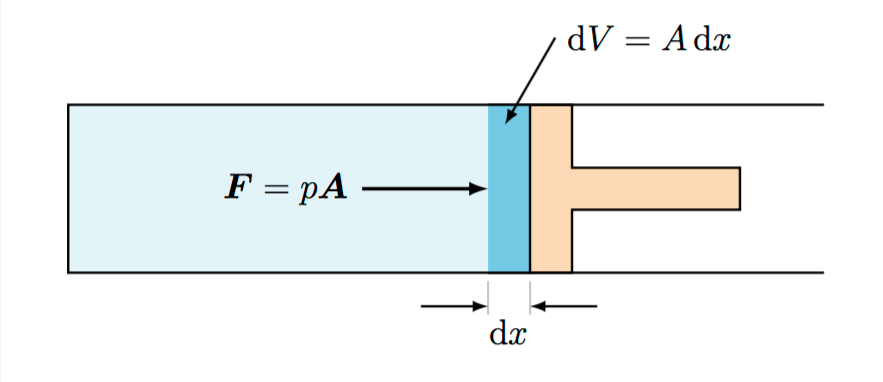
\includegraphics[width=200pt]{images/kolben}
\end{center}

Wenn der Kolben eine Verschiebung $dx$ nach rechts ausf{\"u}hrt, ist die \underline{am Gas} geleistete Arbeit gleich
\begin{equation*}
	dW = -Fdx = -(pA)dx \qquad\text{mit Einheiten}\qquad	 J = -N\cdot m = -(Pa\cdot m^2)m
\end{equation*}
Beachte das Vorzeichen. Die innere Energie des Gases nimmt ab, wenn es sich expandiert. \newline

\subsubsection{Arbeit der Expansion}
Somit ist die geleistete Arbeit eines expandierenden Gases gleich

\begin{equation*}
	dW = -pdV \qquad\text{mit Einheiten}\qquad J = -Pa\cdot m^3
\end{equation*}
Wenn das Volumen eines Gases von $V$ bis $V + dV$ expandiert, ist die \underline{am Gas} geleistete Arbeit gleich $-pdV$. Die \underline{vom Gas} am Kolben geleistete Arbeit ist jedoch gleich $+pdV$.

\subsubsection{Isochore Zustands{\"a}nderung}

W{\"a}hrend dem isochoren Prozess bleibt das textbf{Volumen konstant} ($dV = 0$). Bei so einem Prozess wird die zugef{\"u}hrte W{\"a}rmemenge $dQ$ vollst{\"a}ndig in zus{\"a}tzliche innere Energie des Gases verwandelt. Die Temperatur des Gases erh{\"o}ht sich.
\begin{equation*}
	C_V = \frac{dQ}{dT} = \frac{dU}{dT} = \frac{3}{2	}Nk
\end{equation*}

\subsubsection{Isobare Zustands{\"a}nderung}

Bei isobaren Zustands{\"a}nderungen wird der \textbf{Druck $p$ konstant} gehalten. W{\"a}hrend einer Expansion des Gases muss die Temperatur des Gases erh{\"o}ht oder den Beh{\"a}lter mit zus{\"a}tzlichem Gas gef{\"u}llt werden, damit der Druck konstant bleibt. \newline
Die zugef{\"u}hrte W{\"a}rmemenge verteilt sich also auf die Erw{\"a}rmung und Expansion:
\begin{equation*}
	W = -p(V_e - V_a)
\end{equation*}

\subsubsection{Isotherme Ausdehnung}

Bei einer isothermen Expansion wird die \textbf{Temperatur $T$ des Gases konstant}($dT = 0$) gehalten. Bei einer Expansion nimmt die innere Energie ab. Es folgt also, dass bei einer Expansion W{\"a}rme zugef{\"u}hrt werden muss, um die Temperatur konstant zu halten. \newline
Da die Temperatur des Gases konstant ist, wird die gesamte zugef{\"u}hrte W{\"a}rme in mechanische Arbeit umgewandelt. \newline

F{\"u}r ein ideales Gas gilt also:
\begin{equation*}
	Q = -W = nRT\ln(\frac{V_2}{V_1}) = \int_{V_1}^{V_2}pdV
\end{equation*}

\subsubsection{Adiabatische Ausdehnung}

Bei einer adiabatischen Ausdehnung wird \textbf{keine W{\"a}rme ausgetauscht} ($dQ = 0$).\newline
In einem thermisch isolierten Beh{\"a}lter gilt: Weil das Gas keine W{\"a}rme aufnehmen oder abgeben kann, ist die geleistete Arbeit gleich der Abnahme der inneren Energie $U$. \newline
Es folgt, dass w{\"a}hrend einer adiabatischen Expansion die \textbf{Temperatur des Gases abnimmt}. Die im Gas gespeicherte W{\"a}rmeenergie wird in mechanische Arbeit umgewandelt. \newline
Bei einer adiabatischen Expansion nimmt der Druck $p$ st{\"a}rker ab als bei der isothermen Expansion mit gleicher Volumenzunahme, weil gleichzeitig die Temperatur $T$ abnimmt und $pV = NkT$ gilt.

\begin{equation*}
	\ln(T) + (\gamma - 1) \ln(V) = konst. \Rightarrow TV^{\gamma - 1} = konst.
\end{equation*}

Daraus folgt:
\begin{equation*}
	\frac{pV}{Nk}V^{\gamma-1} = konst. \Rightarrow pV^\gamma = konst.
\end{equation*}

Die vom Gas geleistete Arbeit ist gleich der Fl{\"a}che unter der Kurve im $pV$-Diagramm. Sie ist kleiner als bei einer isothermen Expansion.

\subsection{W{\"a}rmemaschine}

Eine W{\"a}rmemaschine \textbf{wandelt W{\"a}rme in mechanische Arbeit} um. Jede Maschine enth{\"a}lt eine Substanz (das Arbeitsmedium). \newline
In einer \textbf{periodischen W{\"a}rmemaschine} wird ein Kreislauf durchgef{\"u}hrt, die Maschine arbeitet periodisch. Das Arbeitsmedium nimmt bei der h{\"o}heren Temperatur $T_W$ die W{\"a}rme $Q_W$ auf, verrichtet deine Arbeit $W$ und gibt bei der tieferen Temperatur $T_K$ die W{\"a}rme $Q_K$ ab. (W{\"a}rmepumpe funktioniert umgekehrt: nimmt bei tieferen Temperatur $T_K$ W{\"a}rme $Q_K$ auf und gibt unter Ausnutzung der Arbeit $W$ die W{\"a}rme $Q_W$ an das Reservoir der Temperatur $T_W$ ab) \newline

Die W{\"a}rmemaschine leistet Arbeit an ihrer Umgebung:
\begin{equation*}
	|W| = -W = Q_K + Q_W \Rightarrow |W| = |Q_Wt| - |Q_K|
\end{equation*}

\subsection{Zweiter Hauptsatz der Thermodynamik}

\subsubsection{Wirkungsgrad}

Der Wirkungsgrad gibt an, wieviel W{\"a}rme $Q_W$ vom warmen Reservoir aufgenommen werden muss, um die mechanische Arbeit $W$ zu leisten (d.h. $W = Q_W$ und $Q_K = 0 \Rightarrow \varepsilon = 1$).
\begin{equation*}
	\varepsilon = \frac{|W|}{|Q_W|} = \frac{|Q_W|-|Q_K|}{|Q_W|} = 1 - \frac{|Q_K|}{|Q_W|}
\end{equation*}

\subsubsection{Leistungszahl}
Die Leistungszahl ist definiert als das Verh{\"a}ltnis der W{\"a}rme, die dem kalten Reservoir entnommen wurde ($Q_K > 0$), und der zugef{\"u}hrten mechanischen Arbeit ($W > 0$):
\begin{equation*}
	c_L = \frac{Q_K}{W}
\end{equation*}

\subsubsection{Carnotsche W{\"a}rmemaschine}

Der Wirkungsgrad der W{\"a}rmemaschine von Carnot ist
\begin{equation*}
	\varepsilon_{Carnot} = 1 - \frac{|Q_K|}{|Q_W|} = 1 - \frac{T_3}{T_1} \qquad\text{mit}\qquad T_1 > T_3 > 0
\end{equation*}
Er h{\"a}ngt somit nur von den Temperaturen der W{\"a}rmereservoirs ab. \newline

Der Wirkungsgrad aller zwischen zwei Temperatur \textbf{reversibel} arbeitenden W{\"a}rmemaschinen ist gleich gross, und all \textbf{irreversiblen} W{\"a}rmemaschinen haben einen kleineren Wirkungsgrad. \newline

Eine reale W{\"a}rmemaschine kann nie einen h{\"o}heren Wirkungsgrad als die Maschine von Carnot erreichen.
\begin{equation*}
	\varepsilon_{real} < \varepsilon_{Carnot} = 1 - \frac{T_3}{T_1} < 1
\end{equation*}
Der Wirkungsgrad einer idealen, reversiblen W{\"a}rmemaschine von Carnot k{\"o}nnte 100\% nur dann erreichen, wenn $T_1 \rightarrow \infty$ oder $T_3 \rightarrow 0$. W{\"a}re der Wirkungsgrad tats{\"a}chlich 100\%, w{\"u}rde W{\"a}rme vom warmen Reservoir komplett in Arbeit umgewandelt werden. \newline

Es ist unm{\"o}glich, eine periodisch arbeitende Maschine zu bauen, die nichts anderes bewirkt, als durch Abk{\"u}hlung eines W{\"a}rmereservoirs W{\"a}rme in mechanische Arbeit umzuwandeln. \newline

\subsection{Irreversibilit{\"a}t}

Ein nicht-reversibler Prozess ist ein Prozess, der nicht in umgekehrter Richtung ablaufen kann. \newline

\subsubsection{Thermische Irreversibilit{\"a}t}
Ein thermodynamischer Prozess ist reversibel, wenn am Ende des Prozesses, der reversibel durchgef{\"u}hrt wurde, das System und seine lokale Umgebung in ihren Anfangszust{\"a}nden wieder hergestellt werden k{\"o}nnen, ohne {\"a}nderung des Rests des Universums. \newline

\textbf{W{\"a}rmeleitung ist irreversibel}, da man nie beobachtet, wie sich ein K{\"o}rper pl{\"o}tzlich abk{\"u}hlt.

\subsubsection{Mechanische Irreversibilit{\"a}t}

Die \textbf{freie Expansion eines Gases ist irreversibel}. Die Kompression l{\"a}sst sich nicht ausf{\"u}hren, ohne das Universum zu {\"a}ndern. Es ist zwar m{\"o}glich, dass die Molek{\"u}le des Gases zuf{\"a}lligerweise nach einer gewissen Zeit am Anfangsort sind, die Chancen sind jedoch extrem klein. \newline
Die \textbf{isotherme Expansion ist jedoch reversibel}. Die zugef{\"u}hrte W{\"a}rme wird bei der Kompression der Umgebung wieder abgegeben $\Rightarrow$ das Gas und die Umgebung befinden sich wieder in ihrem urspr{\"u}nglichen Zustand.

\section{Elektromagnetismus}

Jedes Elementarteilchen hat eine bestimmte Ladung:
\begin{equation*}
	\text{Elektron:}\quad q_e = -e \quad\text{Proton:}\quad q_p = +e \quad\text{Neutron:}\quad q_n = 0
\end{equation*}
Ladungen sind immer ein Vielfaches der Elementarladung $e$. Sie tr{\"a}gt die Einheit Coulomb. 

\paragraph{Ladungserhaltung:} Die Gesamtladung eines Systems wird immer erhalten.

\subsection{Coulombsche Gesetz}

Das Coulombsche Gesetz beschreibt die Kraft, die eine Ladung $q_1$ auf eine Ladung $q_2$ aus{\"u}bt:
\begin{equation*}
	F_{12} = K\frac{q_1 q_2}{r_{12}^2} \qquad\text{mit Einheiten}\qquad N = \frac{N\cdot m^2}{C^2}\cdot\frac{C^2}{m^2}
\end{equation*}
wobei $r_{12}$ der Einheitsvektor von $q_1$ in Richtung $q_2$ und $K = \frac{1}{4\pi\varepsilon_0}$ Funktion der elektrischen Feldkonstante $\varepsilon_0$ ist.

\begin{center}
	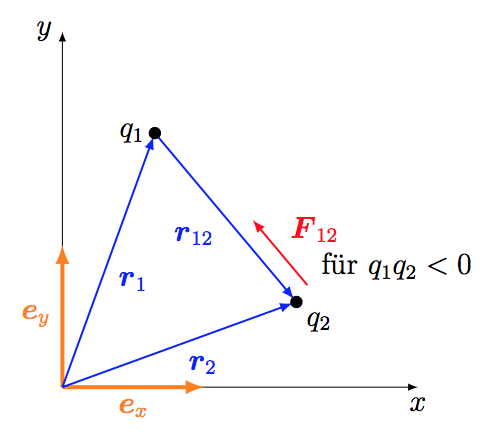
\includegraphics[width=200pt]{images/coulomb}
\end{center}

Da die Gravitationskraft sehr schwach ist, ist sie nur wichtig, wenn der K{\"o}rper elektrisch neutral ist.

\subsection{Elektrische Feld}

Mit dem Ursprung des Koordinatensystems im Mittelpunkt der Punktladung $Q$ ist das elektrische Feld um diesen Punk:
\begin{equation*}
	E(r) \equiv \frac{F(r)}{q} = \frac{1}{4\pi\varepsilon_0}\frac{Q}{r^2}\frac{r}{r} \qquad\text{mit Einheiten}\qquad \frac{N}{C} = \frac{N\cdot m^2}{C^2}\cdot\frac{C}{m^2}
\end{equation*}
Das Feld entspricht der Kraft, die eine Ladung $q$ in diesem Feld erf{\"a}hrt, dividiert durch ihre Ladung. \newline
Die zweite Ladung $q$ sp{\"u}rt das Feld und somit die Kraft:
\begin{equation*}
	F(r) = qE(r)
\end{equation*}
F{\"u}r eine positive Ladung $q$ zeigt die Kraft in die Richtung des Feldes.

\paragraph{Magnetisches vs. elektrisches Feld}\mbox{}\\
\begin{enumerate}
	\item[Richtung] Elektrische Feldlinien beginnen bei positiven Ladungen und enden bei negativen.\newline
		Magnetische Feldlinien bilden geschlossene Schleifen Richtung S{\"u}dpol.
	\item[Kraft] Das elektrische Feld {\"u}bt seine Kraft l{\"a}ngs der Feldlinien aus. \newline
				 Die Kraft des magnetischen Feldes wirkt nur auf bewegte Ladungen und zwar senkrecht zum B-Feld und zur Bewegungsrichtung.
\end{enumerate}

\begin{figure*}[h]
\makebox[\textwidth]{
	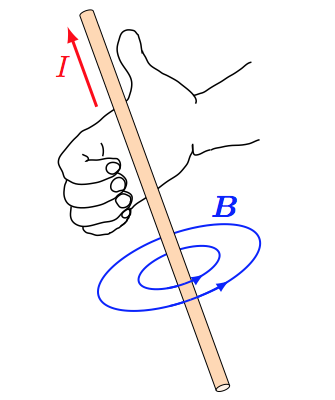
\includegraphics[width=100pt]{images/mf/draht}
	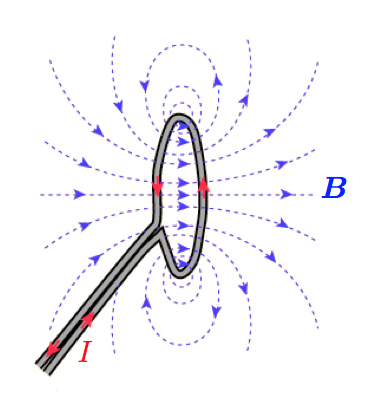
\includegraphics[width=100pt]{images/mf/ring}
	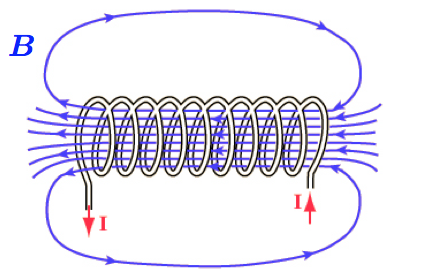
\includegraphics[width=100pt]{images/mf/solenoid}
	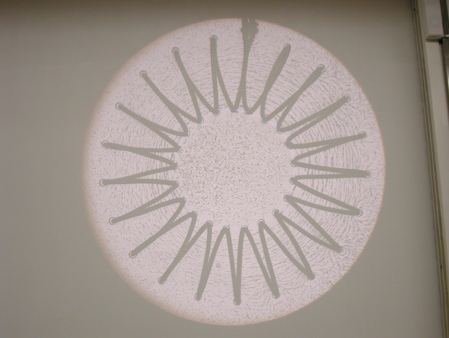
\includegraphics[width=100pt]{images/mf/torus}
}
\captionsetup{labelformat=empty}
\caption{Magnetisches Feld durch einen Draht, Ring, Solenoid, Torus}
\end{figure*}

\subsection{Energie im elektrischen Feld}

\subsubsection{Elektrische potentielle Energie}

Ziehen sich zwei Ladungen an, muss man Arbeit leisten, um deren Abstand zu vergr{\"o}ssern. Stossen sie sich ab, erh{\"a}lt man Arbeit, wenn sich der Abstand vergr{\"o}ssert. \newline
Arbeit wird im System der Ladungen als elektrische potentielle Energie gespeichert:
\begin{equation*}
	E_{pot}^e(r) = \frac{1}{4\pi\varepsilon_0}\frac{q_1 q_2}{r} \qquad\text{mit Einheiten}\qquad J = \frac{N\cdot m^2}{C^2}\cdot\frac{C^2}{m}
\end{equation*}
Wenn sich die Ladungen n{\"a}hern, kann die elektrische potentielle Energie abnehmen oder zunehmen: die Situation h{\"a}ngt vom Vorzeichen des Produkts der Ladungen ab ($q_1 q_2 > 0 \Rightarrow abstossend$). \newline

\subsubsection{Elektrische Potential und Spannung}

\paragraph{Spannung:} Die Kraft, die die Elektronen von der einen Ladung zur anderen drückt.

Das \textbf{elektrische Potential $V$} ist eine Zahl in jedem Punkt des Raums und entspricht der potentiellen Energie f{\"u}r eine Einheitsladung:
\begin{equation*}
	V(r) = \frac{E_{pot}^e(r)}{q} \qquad\text{mit Einheiten}\qquad V = \frac{J}{C}
\end{equation*}

Bewegt sich die Ladung $q$ l{\"a}ngs eines Weges von einem Punkt A zu einem Punkt B, so ist die vom elektrischen Feld geleistete Arbeit:

\begin{equation*}
	W = -q(V(r_B) - V(r_A))
\end{equation*}

Die \textbf{elektrische Spannung} ist gleich dem Potentialunterschied zwischen zwei Punkten:
\begin{equation*}
	U_{1,2} = V(r_1) - V(r_2) = \int_{r_1}^{r_2}E dr \qquad\text{mit Einheit}\qquad V
\end{equation*}

\subsection{Elektrische Ladung im elektrischen und magnetischen Feld}

Eine bewegte Punktladung $Q$ {\"u}bt eine magnetische Kraft auf eine zweite bewegte Ladung $q$ aus. Das magnetische Feld wird von der bewegten Ladung $Q$ erzeugt.

\subsubsection{Lorentz-Kraft}

Die allgemeine elektromagnetische Kraft (Lorentz-Kraft) ist gleich
\begin{equation*}
	F = F_E + F_B = q(E + v \times B) \qquad\text{mit Einheiten}\qquad N = C(\frac{N}{C} + \frac{m}{s}\cdot\frac{N}{C\cdot\frac{m}{s}} = C(\frac{N}{C} + \frac{m}{s}T)
\end{equation*}
wobei $E$ das elektrische Feld und $B$ das magnetische Feld ist. 

Der magnetische Term $F_B$ der Lorentz-Kraft
\begin{enumerate}
	\item ist proportional zur Geschwindigkeit $v$. Auf ein ruhendes Teilchen wirkt keine magnetische Kraft.
	\item wirkt senkrecht zur Bewegungsrichtung und zur Richtung des Feldes.
	\item den Betrag $|F_B| = |q||v||B|sin(\alpha)$ hat, wobei $\alpha$ der Winkel zwischen $v$ und $B$ ist.
\end{enumerate}

\subsubsection{Bewegung im elektrischen Feld}

Das \textbf{Elektronenvolt (eV)} ist gleich der gesamten Energiezunahme, die ein Teilchen mit der ElementarLadung $e$ erf{\"a}hrt, wenn es durch einen Potentialunterschied von 1 Volt beschleunigt wird. \newline

Unter der Wirkung der elektrischen Kraft erf{\"a}hrt ein Teilchen der Ladung $q$ und Masse $m$ die Beschleunigung (f{\"u}r nichtrelativistische Geschwindigkeiten)
\begin{equation*}
	F = qE = \frac{dp}{dt} = ma \Rightarrow q = \frac{q}{m}E
\end{equation*}

\subsubsection{Bewegung im magnetischen Feld}

Da die Wirkung des Magnetfeldes immer senkrecht zur Bewegungsrichtung ist, {\"a}ndert sich bei einem Teilchen nur die Richtung, nicht jedoch den Betrag der Geschwindigkeit. Daher ist die an einem Teilchen von der magnetischen Kraft verrichtete Arbeit immer null. \newline

Das magnetische Feld leistet keine Arbeit an einem Teilchen und hat keinen Einfluss auf dessen kinetische Energie. \newline

Bewegt sich jedoch ein Teilchen genau senkrecht zum Feld bewegt, so beschreibt das Teilchen eine Kreisbahn mit dem Radius $r$: die magnetische Kraft wirkt als eine Zentripetalkraft.

\begin{minipage}{.5\textwidth}
    \begin{equation*}
    qvB = \frac{m\gamma v^2}{r} \Leftrightarrow r = \frac{m\gamma v}{qB}
    \end{equation*}
\end{minipage}%
\begin{minipage}{.5\textwidth}
  	\centering
    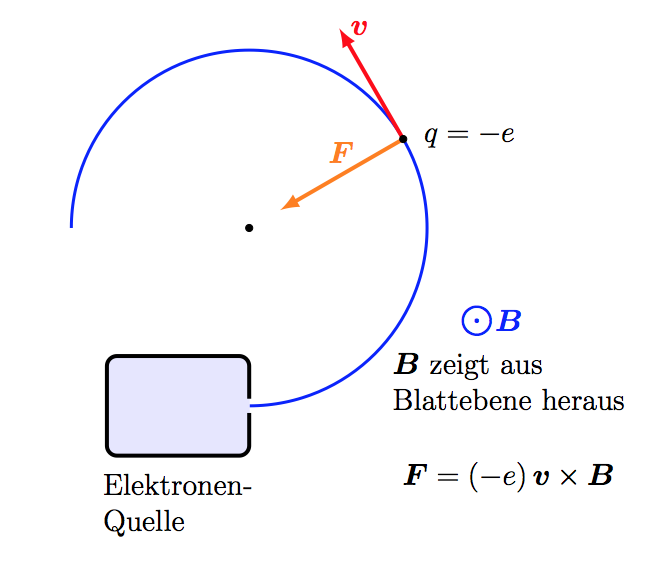
\includegraphics[width=200pt]{images/mf/zentripetalkraft}
\end{minipage}

\subsection{Der elektrische Strom}

\paragraph{Strom:} Anzahl Elektronen pro Zeiteinheit

Wenn der \textbf{Ladungsfluss nicht konstant} ist, so ist die momentane \textbf{elektrische Stromst{\"a}rke $I$} gleich
\begin{equation*}
	I(t) = \frac{dQ}{dt} \qquad\text{mit Einheiten}\qquad A = \frac{C}{s}
\end{equation*}

Die positive Stromrichtung folgt der Flussrichtung der positiven Ladung (historische Konvention).

Ist der \textbf{Ladungsfluss konstant}, so ist die Stromst{\"a}rke gleich
\begin{equation*}
	I = -enAv_D \qquad\text{mit Einheiten}\qquad A = C\cdot\frac{1}{m^3}\cdot m^2\cdot\frac{m}{s}
\end{equation*}
wobei $v_D$ die Driftgeschwindigkeit bezeichnet. Sie ist viel kleiner als die Geschwindigkeit freier Elektronen, da die Elektronen im Leiter oft mit Ionen kollidieren.

Die \textbf{Stromdichte $j$} wird als die Stromst{\"a}rke pro Fl{\"a}che definiert:
\begin{equation*}
	j = \frac{I}{A} \qquad\text{mit Einheiten}\qquad \frac{A}{m^2}
\end{equation*}

Die \textbf{Driftgeschwindigkeit} ist die Geschwindigkeit, die ein Elektron zwischen zwei Ionenst{\"o}ssen erreichen wird.
\begin{equation*}
	v_D = a\tau = -\mu E \qquad\text{mit Einheiten}\qquad \frac{m}{s} = \frac{m}{s^2}s
\end{equation*}
wobei $\mu = \frac{e\tau}{m}$ die Beweglichkeit der Elektronen und $v_D$ die Driftgeschwindigkeit ist. Sie ist proportional zum elektrischen Feld. Die Richtung der Elektronenbewegung ist zur Richtung des Feldes parallel, zeigt jedoch in die entgegengesetzte Richtung.

\subsection{Das Ohmsche Gesetz}

\begin{equation*}
	U_{AB} = RI = (\frac{L}{\sigma A})I \qquad\text{mit Einheiten}\qquad V = (\frac{m}{\frac{A}{V \cdot m}\cdot m^2})A = \Omega \cdot A
\end{equation*}
wobei $L$ die gesamte L{\"a}nge, $R$ der Widerstand und $\sigma$ die Leitf{\"a}higkeit des Leiters ist und $U_{AB}$ die Spannung von A nach B. Die Einheit der Leitf{\"a}higkeit ist $\frac{A}{V\cdot m}$.
\subsection{Kraft auf einem elektrischen Strom}

Die Gesamtkraft, die ein Magnetfeld auf einen Leiter der Querschnittsfl{\"a}che A mit L{\"a}nge L aus{\"u}bt ist:
\begin{equation*}
	F = ALn(-e)v_D \times B = LI \times B
\end{equation*}

Bei \textbf{zwei parallelen Leitern} erfahren die Leiter eine seitlich wirkende Kraft des anderen Leiters:

\begin{equation*}
	F \approx \frac{LI_1I_2}{r} \qquad\text{mit der vektoriellen Beziehung}\qquad F = LI \times B
\end{equation*}
Fliesst der Strom bei beiden Leitern in die selbe Richtung, so ziehen sich die Leiter gegenseitig an.

\subsection{Elektrische Kapazität und Kondensatoren}

In einem \textbf{Kondensator} wird Energie in einem elektrischen Feld in Form von potenzieller Energie gespeichert. 
\begin{equation*}
	Q = CV \qquad\text{mit Einheiten}\qquad C = FV = \frac{C}{V}V
\end{equation*}
wobei $C$ die Kapazität des Kondensators in Farad ist. Die Ladung $Q$ (Betrag der Ladung einer Platte) und die Potenzialdifferenz $V$ sind zueinander proportional. \newline

Die geleistete Arbeit zur Aufladung des Kondensators kann man als Energie wieder entnehmen:
\begin{equation*}
	E = \frac{Q^2}{2C} = \frac{1}{2}CV^2
\end{equation*}

\subsection{Theorem von Gauss}

Die Divergenz des Feldes in jedem Punkt ist gleich dem Fluss, der das den Punkt umgebende Volumenelement $dxdydz$ verlässt, dividiert durch dieses Volumen.
\begin{equation*}
	d\Phi_{tot}(x,y,z) = {\nabla\cdot F(x,y,z)}dxdydz
\end{equation*}

Der gesamte Fluss $\Phi_{tot}$, der aus einem Volumen $V$ austritt, ist gleich
\begin{equation*}
	\Phi_{tot} = \oiint_{A=\partial V}F \cdot dA = \iiint _V(\nabla\cdot F)dV
\end{equation*}
wobei der erste Term dem \textbf{Flächenintegral} und der zweite dem \textbf{Volumenintegral} entspricht. $A$ ist die Oberfläche, die das Volumen $V$ einschliesst.

\subsection{Theorem von Stokes}

Dieses Theorem setzt das Linienintegral über die geschlossene Kurve $C$ mit dem Flächenintegral über die Fläche $A$ in Beziehung: \newline
Das Linienintegral eines Feldes $F$ über eine geschlossene Kurve $C$ ist gleich dem Flächenintegral der Rotation des Feldes über die Fläche $A$, wobei $A$ von $C$ umrandet wird.

\begin{equation*}
	\oint _C F \cdot dr = \iint _A (\nabla \times F) \cdot dA
\end{equation*}

wobei $C$ die geschlossene Kurve ist, die die Fläche $A$ einschliesst.

\subsection{Ladungs- und Stromdichte}

\subsubsection{Ladungsdichte}

Die \textbf{Raumladungsdichte} ist wie folgt definiert:
\begin{equation*}
	\rho(r) = \frac{dq}{dV}
\end{equation*}
wobei $dq$ die infinitesimale Ladung im Volumenelement $dV$ ist. \newline

Die gesamte Ladung eines Körpers ist somit gleich
\begin{equation*}
	Q = \int dq = \iiint _V \rho(r) dV = \iiint _V \rho (x,y,z) dx dy dz
\end{equation*}

\subsubsection{Vektorielle Stromdichte}

Der Strom, der durch die Fläche $A$ fliesst, ist gleich
\begin{equation*}
	I = \iint _A j(r) \cdot dA
\end{equation*}

Die \textbf{Kontinuitätsgleichung} sagt voraus, dass wenn sich die elektrische Ladung in einem Punkt $r$ ändert, muss in diesem Punkt ein elektrischer Strom fliessen:
\begin{equation*}
	\frac{\partial\rho (r)}{\partial t} + \nabla\cdot j(r) = 0
\end{equation*}

\subsection{Maxwellgleichungen}
\begin{equation*}
\begin{split}
	\varepsilon _0 (\nabla\cdot E) & = \rho \\
	(\nabla\cdot B) & = 0 \\
	\nabla\times E & = -\frac{\partial B}{\partial t} \\
	\nabla\times B & = \mu _0 j + \varepsilon _0 \mu _0 \frac{\partial E}{\partial t}	
\end{split}
\end{equation*}
wobei 
\begin{enumerate}
	\item [$E(x,y,z,t)$] das elektrische Vektorfeld
	\item [$B(x,y,z,t)$] das magnetische Vektorfeld
	\item [$\rho(x,y,z,t)$] die Ladungsdichte
	\item [$j(x,y,z,t)$] die Stromdichte
\end{enumerate}

\end{document}
